\documentclass[tikz,border=6pt]{standalone}
\usepackage{ctex}
\usepackage{amsmath}
\usetikzlibrary{arrows.meta,positioning,shapes.geometric}

\begin{document}
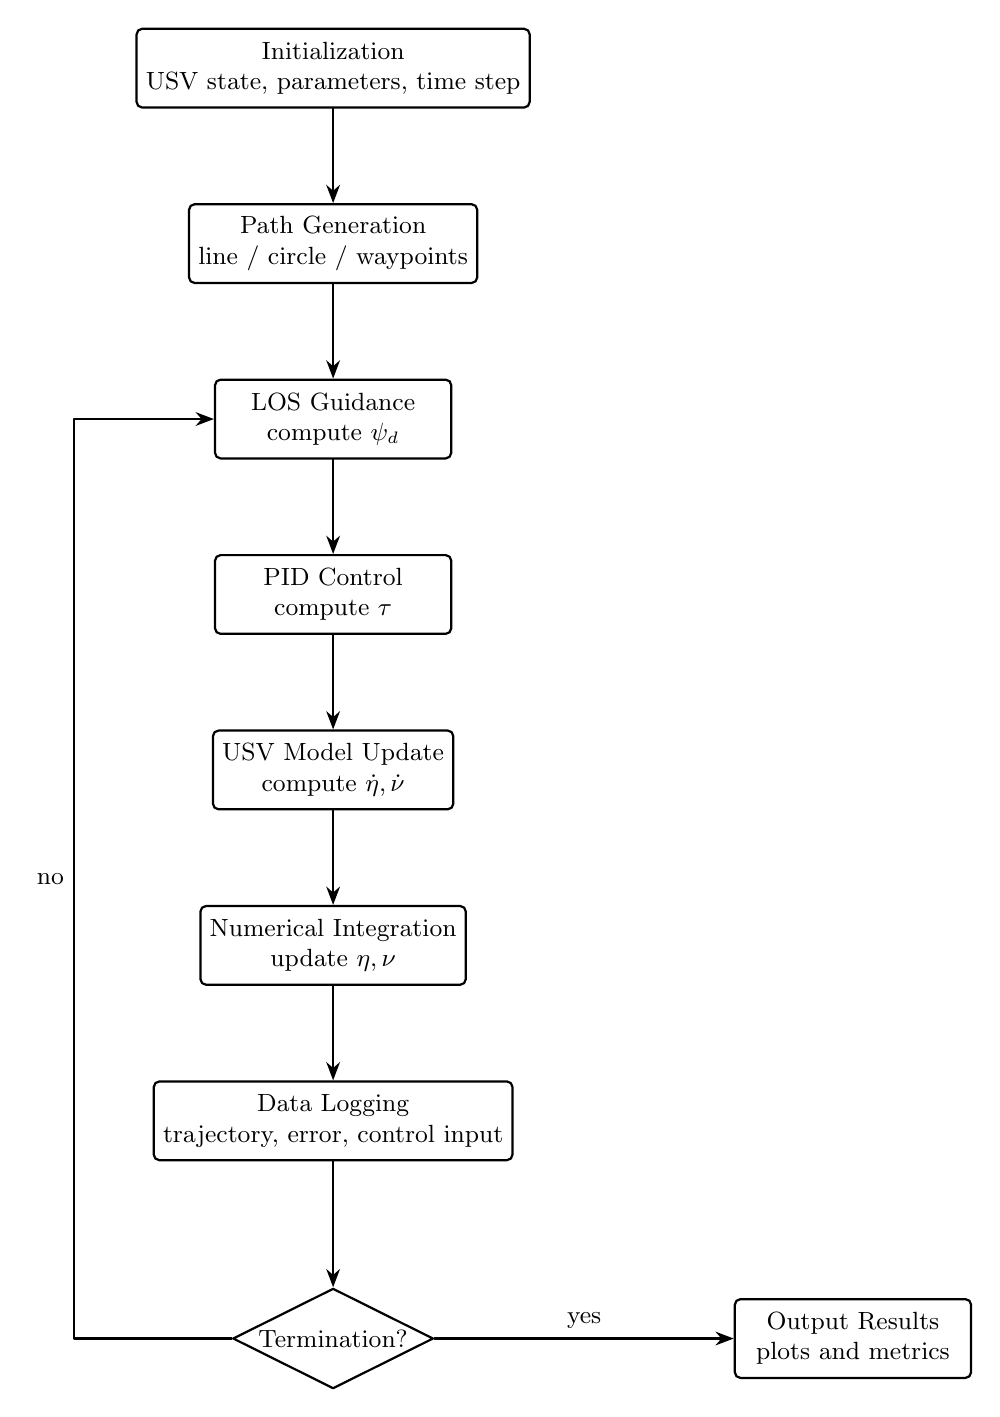
\begin{tikzpicture}[
    >=Stealth,
    font=\small,
    line join=round,
    line cap=round,
    block/.style={
        draw,
        thick,
        rectangle,
        rounded corners=2pt,
        minimum width=3.0cm,
        minimum height=1.0cm,
        align=center
    },
    decision/.style={
        draw,
        thick,
        diamond,
        aspect=2.0,
        align=center,
        inner sep=1pt
    },
    signal/.style={->, thick}
]

% =========================
% Nodes
% =========================
\node[block] (start) {Initialization\\USV state, parameters, time step};

\node[block, below=1.2cm of start] (path) {Path Generation\\line / circle / waypoints};

\node[block, below=1.2cm of path] (los) {LOS Guidance\\compute $\psi_d$};

\node[block, below=1.2cm of los] (pid) {PID Control\\compute $\tau$};

\node[block, below=1.2cm of pid] (model) {USV Model Update\\compute $\dot{\eta},\dot{\nu}$};

\node[block, below=1.2cm of model] (intg) {Numerical Integration\\update $\eta,\nu$};

\node[block, below=1.2cm of intg] (log) {Data Logging\\trajectory, error, control input};

\node[decision, below=1.6cm of log] (judge) {Termination?};

\node[block, right=3.8cm of judge] (endnode) {Output Results\\plots and metrics};

% =========================
% Main flow
% =========================
\draw[signal] (start) -- (path);
\draw[signal] (path) -- (los);
\draw[signal] (los) -- (pid);
\draw[signal] (pid) -- (model);
\draw[signal] (model) -- (intg);
\draw[signal] (intg) -- (log);
\draw[signal] (log) -- (judge);

% =========================
% Decision branches
% =========================
\draw[signal] (judge) -- node[above] {yes} (endnode);

\draw[signal] (judge.west) -- ++(-2.0,0) |- node[pos=0.25,left] {no} (los.west);

\end{tikzpicture}
\end{document}